\documentclass[11pt]{article}
%\documentclass{beamer}
\usepackage[utf8]{inputenc}  
\usepackage[T1]{fontenc}
\usepackage[francais]{babel}
\usepackage{amsmath,textcomp,amssymb,geometry,graphicx,enumerate}
\usepackage{algorithm} % Boxes/formatting around algorithms
\usepackage[noend]{algpseudocode} % Algorithms
\usepackage{hyperref}
\usepackage{stmaryrd}
\hypersetup{
    colorlinks=true,
    linkcolor=blue,
    filecolor=magenta,      
    urlcolor=blue,
}

\def\Name{Amauri López Cabrera}  % Your name
\def\SID{Lycée Lakanal}
\def\Login{} % Your login (your class account, cs170-xy)
\def\Homework{N} % Number of Homework
\def\Session{}


\title{Absorción y Esparcimiento de luz por partículas pequeñas}
\author{\Name{} \texttt{\Login}}
\markboth{\Session\   \Name}{\Session\  \Name, \texttt{\Login}}
\pagestyle{myheadings}
\date{}

\newenvironment{qparts}{\begin{enumerate}[{(}a{)}]}{\end{enumerate}}
\def\endproofmark{$\Box$}
\newenvironment{proof}{\par{\bf Proof}:}{\endproofmark\smallskip}

\textheight=9.5in
\textwidth=7in
\topmargin=-.5in
\oddsidemargin=0.001in
\evensidemargin=0.001in
\begin{document}
\section*{4.4 Absorción y esparcimiento por una esfera[1]}
\subsection*{4.4.2 Ejemplos de extinción: Interferencia y estructura ondulatoria, redeening (enrojecimiento)}

Ahora, pasaremos del desarrollo matemático para considerar algunos ejemplos de extinción. Una discusión mas completa sobre la extinción se da en el capitulo 11. Los métodos computacionales utilizados para generar este tipo de ejemplos será discutido en capítulos posteriores. Para nuestro breve ejemplo de extinción escogimos gotas de agua en el aire; las constantes ópticas dependientes de la longitud de onda-desde radio hasta UV-que se utilizan en este calculo están dados en el Capitulo 10.

\begin{figure}[H]
\centering
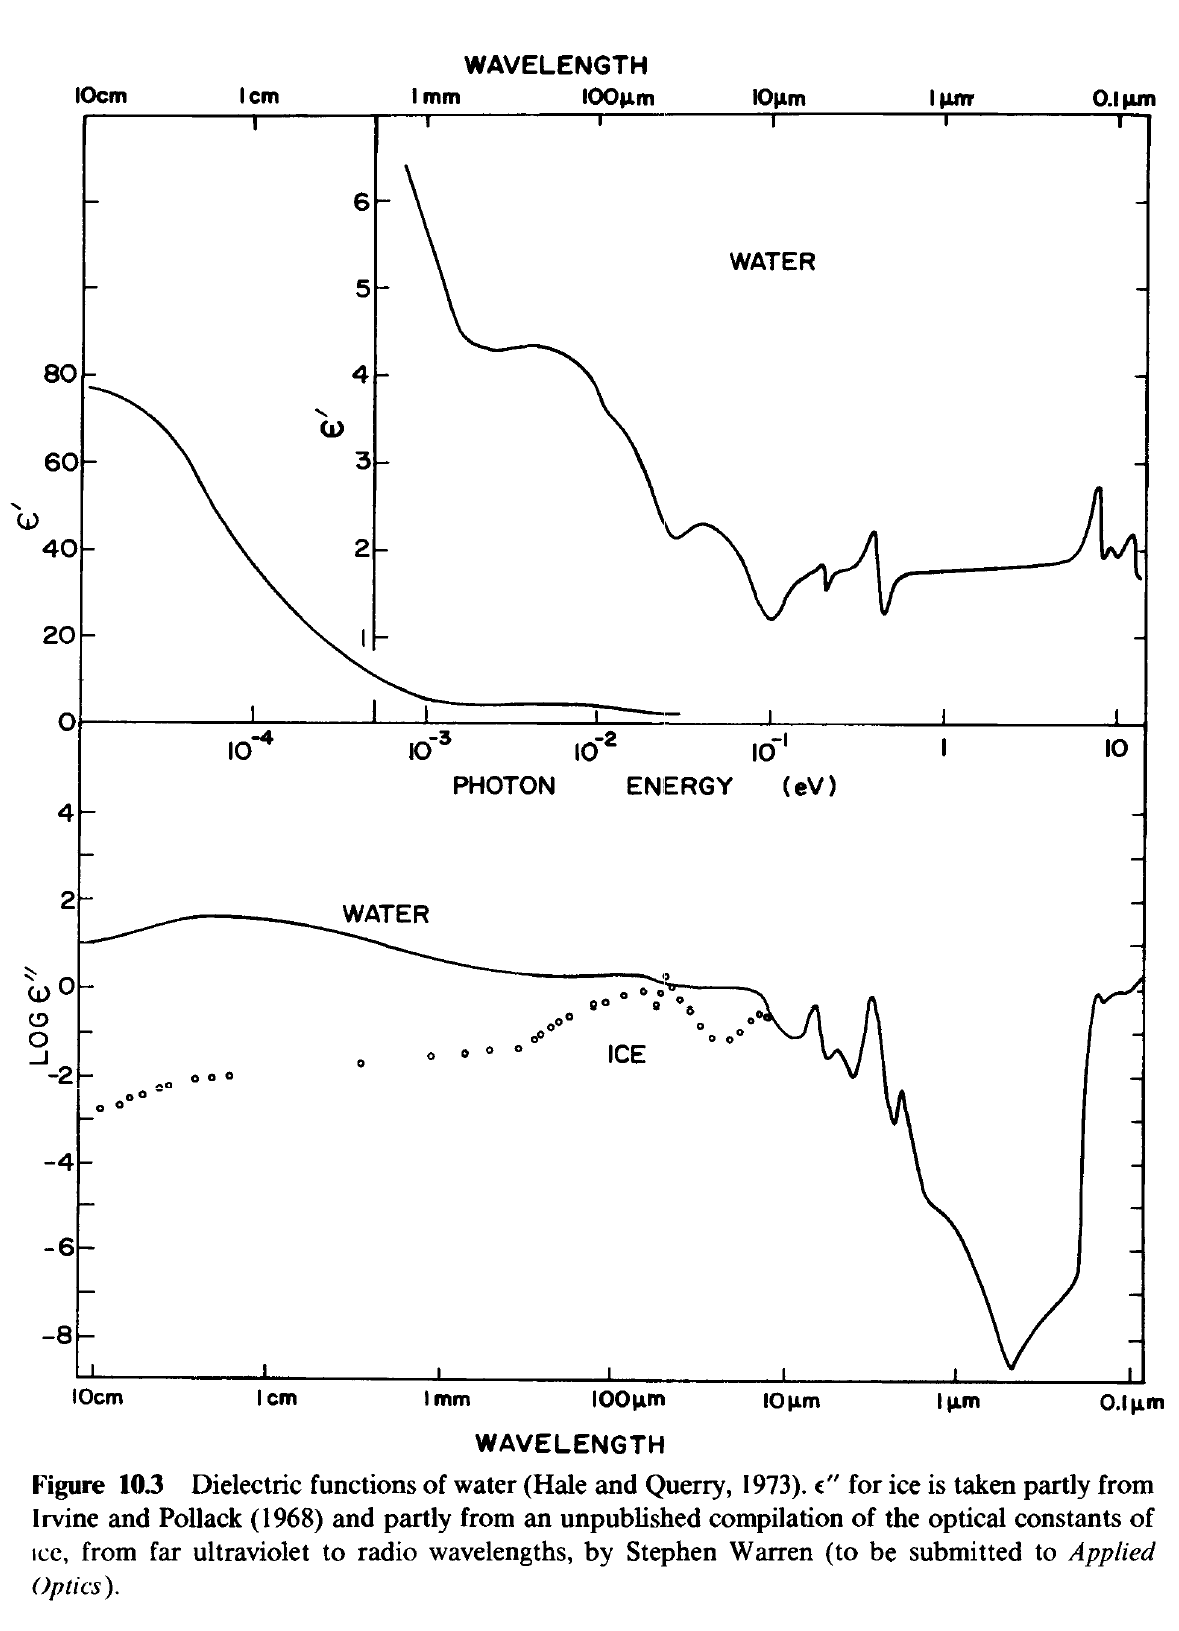
\includegraphics[scale=0.4]{1.png}
\label{fig:p0}
\end{figure}

La imagen 1 muestra las funciones dielectricas calculadas de los índices de refracción tabulados por Hale and Querry; las constantes ópticas a longitudes de onda corta 0.2 $\mu$m fueron tomadas directamente del trabajo de Kerr et al.(1972)
\\ \\
La absorción electrónica por el $H_{2}O$ se da sobre el continuo entre 1 y 100 $\mu$m. También podemos observar que el punto de menor absorción en el espectro cae en la región visible, donde $\epsilon$'' donde cae a menos de 10$^{-8}$.
\\ \\

\begin{figure}[H]
\centering
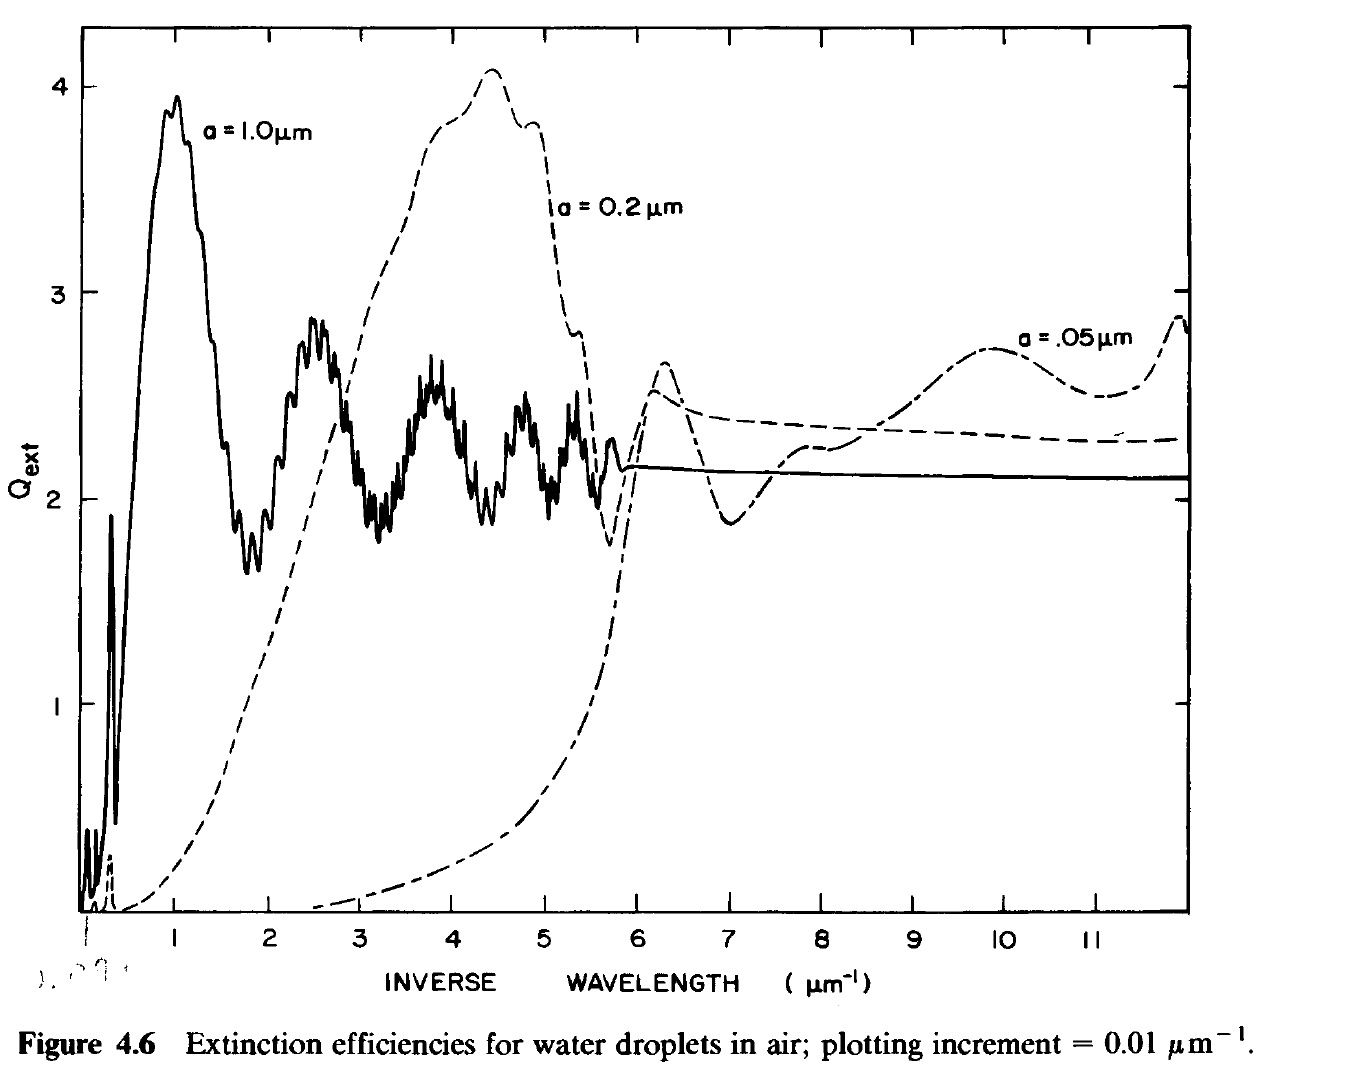
\includegraphics[scale=0.5]{2.png}
\label{fig:p0}
\end{figure}

Curvas de extinción calculadas para tres diferentes radios se muestran en la figura 2, donde la eficiencia de extinción esta graficada como función del inverso de función de onda $\frac{1}{\lambda}$

\begin{equation}
    Q_{0} = \frac{C_{ext}}{\pi a^{2}}
\end{equation}

Esto de alguna forma es un método poco convencional para mostrar la extinción, puede ocasionar que algunos lectores se tambaleen de terror, particularmente cuando se observa que las curvas de la figura 2 muestran marcadas desviaciones de aquellas que se encuentran mas comúnmente; las eficiencias de extinción se muestran usualmente como funciones de $x$ para un índice de refracción fijo m, una practica consagrada por tradición.
Aunque el método tradicional de mostrar la extinción no es necesariamente incorrecto, puede llevar a confusiones: $x$ y m son matemáticamente  variables independientes pero físicamente no son independientes. Este hecho elemental a menudo se pierde de vista cuando se considera que $x$ es simplemente una variable adimensional que es indiferente a si cambia debido a la longitud de onda variable o al radio.Si la longitud de onda varia también variara m$:$ ningún material tiene constantes ópticas independientes de la longitud de onda excepto por un rango muy angosto. Desafortunadamente, en algunas áreas donde la teoría de esparcimiento ha sido aplicada, la plena realización de esto se ha dado lentamente; el resultado, falsas conclusiones basadas en razonamientos erróneos.
Uno de los temas centrales de este libro es que la comprensión completa de la dispersión de la luz y la absorción por parte de las partículas requiere comprender las propiedades ópticas de la materia en bulto. La razón por la cuál se presenta de esa forma la gráfica de extinción tiene que ver mas con la conveniencia que fidelidad a la realidad física: es relativamente fácil calcular $Q_{ext}$ como función de x con m fijo. Las curvas de la figura 2 requieren un esfuerzo considerable$:$ para cada una de las longitudes de onda que utilizamos para el calculo se deben utilizar las correctas propiedades ópticas. El esfuerzo computacional per se requerido para graficar $Q_{ext}$ se oscurece por la labor de compilar las constantes ópticas de muchas fuentes y de forma adecuada llevar acabo una interpolación de los datos obtenidos. La recompensa de esto es una idea física de mayor precisión sobre la extinción.
\\ \\ 

En la región donde el agua absorbe menos es entre los 0.5 y 5 $\mu m^{-1}$ la gota de agua con 1.0$\mu m$ de radio muestra varias características. 
\\ \\
\textbf{1}: una serie de máximos y mínimos  regularmente espaciados llamados estructura de interferencia, los cuales oscilan alrededor del valor 2
\\ \\
\textbf{2}: estructura fina irregular llamada estructura ondulatoria.
\\ \\
\textbf{3}: incremente monotónico de la extinción para longitudes de onda tal que $a < \lambda$ ; consideraremos cada una de estos puntos a la vez.
\\ \\
Para x grandes $(>> n^{2})$ y |mx| el numerador de $a_{n}$ es aproximadamente 

\begin{equation}
    \frac{(m-1)sen[x-n\pi/2]cos[mx-n\pi/2]+msen[x(m-1)]}{x}
\end{equation}
Con la misma aproximación el numerador de $b_{n}$ es

\begin{equation}
    \frac{(1-m)sen[x-n\pi/2]cos[mx-n\pi/2]+sen[x(m-1)]}{mx}
\end{equation}

Para obtener las dos ecuaciones anteriores de los coeficientes $a_{n}$ y $b_{n}$ utilizamos las relaciones asintóticas 

\begin{equation}
    \psi(\rho) \sim sen(\rho-n\pi/2) \hspace{2cm} (|\rho|>> n^{2})
\end{equation}


\begin{figure}[H]
\centering
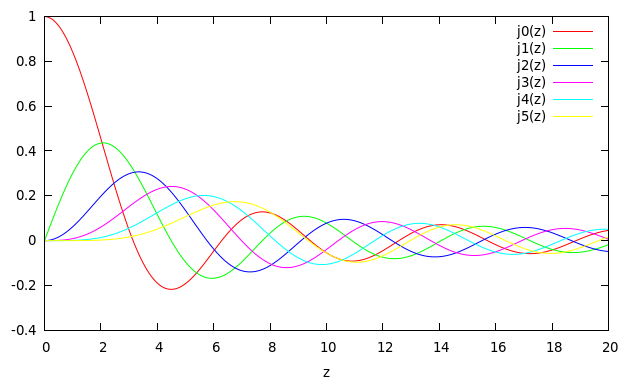
\includegraphics[scale=0.6]{3.png}
\label{fig:p0}
\end{figure}


\subsection*{Coeficiente $a_{n}$}
Sustituyendo la aproximación en el numerador del coeficiente de Mie tenemos:

\begin{equation}
 \frac{mSen[mx-n\pi/2]Cos[x-n\pi/2]-Sen[x-n\pi/2]Cos[mx-n\pi/2]}{x}
\end{equation}

Nos fijamos ahora en el primer término del numerador

\begin{equation}
  mSen[mx-n\pi/2]Cos[x-n\pi/2]
\end{equation}
Desarrollando 
\begin{equation}
(mSen[mx]Cos[n\pi/2]-mSen[n\pi/2]Cos[mx])*(Cos[x]Cos[n\pi/2]+Sen[x]Sen[n\pi/2])
\end{equation}
Multiplicando
\begin{equation}
mSen[mx]Cos[n\pi/2]^2Cos[x]+mSen[mx]Sen[x]Cos[n\pi/2]Sen[n\pi/2]
\end{equation}
\begin{equation*}
-mCos[x]Cos[mx]Cos[n\pi/2]Sen[n\pi/2]-mSen[x]Cos[mx]Sen[x-n\pi/2]^2
\end{equation*}
El primer y último termino
\begin{equation}
mSen[mx]Cos[n\pi/2]^2Cos[x]-mSen[x]Cos[mx]Sen[x-n\pi/2]^2
\end{equation}
Toman la forma
\begin{equation*}
mSen[mx]Cos[n\pi/2]^2Cos[x]-mSen[x]Cos[mx]Sen[x-n\pi/2]^2
\end{equation*}
equivalentemente
\begin{equation*}
mSen[mx](1-Sen[x-n\pi/2]^2)Cos[x]-mSen[x]Cos[mx](Cos[n\pi/2]^2-1)
\end{equation*}
Expandiendo
\begin{equation*}
mSen[mx]Cos[x]-mSen[mx]Sen[x-n\pi/2]^2)Cos[x]-mSen[x]Cos[mx]Cos[n\pi/2]^2-mSen[x]Cos[mx]
\end{equation*}
Recordemos que esta expresión es equivalente al primer y último término de la ecuación (8), de esta forma la ecuación (8) toma la forma



\begin{equation}
mSen[x]Cos[mx]Cos[n\pi/2]^2+mSen[mx]Sen[x]Cos[n\pi/2]Sen[n\pi/2]-mCos[x]Cos[mx]Cos[n\pi/2]Sen[n\pi/2]
\end{equation}
\begin{equation*}
-mSen[mx]Sin[x-n\pi/2]^2Cos[x]+mSen[mx]Cos[x]-mSen[x]Cos[mx]    
\end{equation*}
Simplificando
\begin{equation}
    (mSen[x]Cos[n\pi/2]-mSen[n\pi/2]Cos[x])*(Cos[mx]Cos[n\pi/2]+Sen[x-n\pi/2]Sen[mx])
\end{equation}
\begin{equation*}
+mSen[mx]Cos[x]-mSen[x]Cos[mx]
\end{equation*}
Volviendo a simplificar
\begin{equation}
mSen[x-n\pi/2]Cos[x-n\pi/2]+mSen[mx-x]
\end{equation}
La ecuación (12) es simplemente otra forma de escribir la ecuación (6), sustityendo (12) en (5) tenemos
\begin{equation}
   \frac{mSen[x-n\pi/2]Cos[x-n\pi/2]+mSen[mx-x] -Sen[x-n\pi/2]Cos[x-n\pi/2]}{x}
\end{equation}

si agrupamos obtenemos 

\begin{equation}
    \frac{(m-1)Sen[x-n\pi/2]cos[mx-n\pi/2]+mSen[x(m-1)]}{x}
\end{equation}
\subsection*{Coeficiente $b_{n}$}
Para el coeficiente $b_{n}$ tenemos, bajo la misma aproximación que el numerador tiene la forma 
\begin{equation}
    \frac{Sen[mx-n\pi/2]Cos[x-n\pi/2]-mCos[mx-n\pi/2]Sen[x-n\pi/2]}{x}
\end{equation}
Nuevamente nos fijamos en elprimer término del numerador de esta expresión
\begin{equation}
   Sen[mx-n\pi/2]Cos[x-n\pi/2]
\end{equation}
La similitud con la ecuación (6) nos permite escribir la ecuación 15 de la siguiente forma (usando (12) pero sin el factor de m)
\begin{equation}
    \frac{Sen[x-n\pi/2]Cos[x-n\pi/2]+Sen[mx-x]-mCos[mx-n\pi/2]Sen[x-n\pi/2]}{x}
\end{equation}
y esto es lo mismo que
\begin{equation}
    \frac{(1-m)Cos[mx-n\pi/2]Sen[x-n\pi/2]+Sen[mx-x]}{x}
\end{equation}
























Notemos que tanto en el numerador de $a_{n}$ y $b_{n}$ tenemos el termino en común sen[x(m-1)], el cual es independiente de n; por tanto, esperamos que el máximo de la sección transversal de extinción este aproximadamente determinado por el máximo de esta función, los cuales ocurren para

\begin{equation}
    x(m-1)=(2p+1)\pi/2
\end{equation}

donde p es un entero. Por tanto, la separación $\Delta (1/\lambda)$ entre los máximos de sen[x(m-1)], sobre una región de la longitud de onda donde m sea aproximadamente constante y real es $\frac{a(m-1)}{2}$. Para longitudes de onda en el visible la m del agua se toma como 1.33; por tanto, esperamos que los máximos de la sección transversal para una gota con radio 1.0$\mu m$ estén separados por 1.5$\mu m^{-1}$. El origen del nombre $"$estructura de interferencia$"$ aplicado a este espaciamiento entre los picos de extinción recae en la interpretación de la extinción como la interferencia entre la luz incidente y el esparcimiento de luz en la dirección de propagación. Si ahora adoptamos el punto de vista de la óptica elemental, la diferencia de fase $\Delta \phi$ entre un rayo que atraviesa una esfera transparente sin desviarse y un rayo que atraviesa el mismo camino fuera de la esfera es:

\begin{equation}
    \Delta \phi = \frac{2\pi}{\lambda}2a(N_{1}-N)=2x(m-1)
\end{equation}

La condición para que se presente la interferencia destructiva entre estos dos ratos es 

\begin{equation}
    \Delta \phi = (2p+1)\pi 
\end{equation}

o, equivalentemente 

\begin{equation}
    x(m-1)=(2p+1)\pi/2
\end{equation}

la cual es la misma condición obtenida para los numeradores de $a_{n}$ y $b_{n}$. 
Aplazaremos la discusión detallada de la estructura de ondulación, la cual es considerablemente mas complicada tanto matemática como físicamente que la estructura de interferencia. Basta con decir por el momento que la estructura de ondulación tiene sus orígenes en las raíces de la ecuaciones trascendentales, las condiciones para que los denominadores de los coeficientes de esparcimiento desaparezcan.

\begin{equation}
\frac{[xh_{n}^{1}(x)]'}{h_{n}^{1}(x)}\simeq \frac{\mu_{1}[mxj_{n}(mx)]'}{\mu m^2 j_{n}(mx)}
\end{equation}
\begin{equation}
\frac{[xh_{n}^{1}(x)]'}{h_{n}^{1}(x)}\simeq \frac{\mu [mxj_{n}(mx)]'}{\mu_{1} j_{n}(mx)}
\end{equation}

Tanto la estructura de interferencia como la estructura ondulatoria, disminuyen significativamente cuando la absorción se vuelve mayor, para este caso si $1/\lambda$ es mayor que 6.0$\mu m^{-1}$ para una gota de agua de radio 0.05-$\mu m$ y 0.3$\mu m^{-1}$ para una gota de agua de radio 1.0-$\mu m$ no tenemos estructura de interferencia ni estructura ondulatoria pero si tenemos picos de absorción de bulto. Esto ilustra el hecho que la absorción domina sobre el esparcimiento cuando la razón $a/\lambda$ es pequeña y si hay alguna absorción apreciable por parte del bulto. Un fenómeno mas familiar es el $"$enrojecimiento$"$ de la luz blanca al pasar por una colección de pequeñas partículas. Esto puede demostrarse fácilmente poniendo unas cuantas gotas de leche en un contenedor de agua: un haz de luz blanca colimado toma un color rojizo después de la transmisión a través de la suspensión, esto ya que la longitud de onda de la luz azul se extingue de forma mas eficiente que la longitud de onda de la luz roja. El aumento de la extinción hacia longitudes de onda más cortas es una característica general de partículas(no absorbentes) pequeñas comparadas con la longitud de onda, esto se exhibe en las curvas de extinción de la figura 2 para las dos partículas de radio pequeño. 
\\ \\
Todos estamos familiarizados con las puestas de sol de color rojo y naranja, ocasionadas en parte por el esparcimiento molecular. Partículas pequeñas pueden mejorar el enrojecimiento del atardecer. Periodos largos de actividad volcánica incrementan la belleza de los colores de atardecer por periodos de hasta un año principalmente por las partículas en la atmósfera; altos niveles de contaminación tienden a incrementar el enrojecimiento.
\\ \\
El enrojecimiento debido a la extinción por partículas pequeñas no esta limitado al entorno terrestre. Partículas de polvo entre las estrellas extinguen la luz azul de forma mas eficiente que la roja,por tanto, la luz de la estrella transmitida a través de este polvo esta enrojecida.
Este efecto es tan confiable y uniforme cuando se promedia a lo largo de muchos miles de años luz que puede usarse para medir distancias a las estrellas en nuestra galaxia. Una estrella $"$altamente enrojecida$"$ (como se dice en la jerga), es aquella que tiene una alta cantidad de materia interestelar entre esta y el observador. De la figura 2 es obvio que la extinción depende del tamaño de la partícula. De echo, la dependencia en el tamaño nos provee con la evidencia de que los granos de materia interestelar son de tamaño submicroscópico en su mayoría. Sin embargo en el laboratorio, otros tipos de mediciones tales como esparcimiento angular son preferibles para determinar el tamaño de las partículas.
\\ \\
El enrojecimiento ocurre siempre que las partículas sean pequeñas comparadas con la longitud de onda sin importar el tamaño de la distribución. El efecto opuesto, $"$azulado$"$, puede observarse en las frecuencias altas de los picos de extinción. El  $"$azulado$"$ es altamente dependiente en el tamaño de la distribución y tiende a desaparecer así como la estructura de interferencia cuando el radio de la partícula incrementa. Por lo tanto, el  $"$azulado$"$ de la luz de sol por partículas en la atmósfera es raro pero tampoco imposible: Luna azul. Después de la gran explosión del volcán Krakatoa se observo que el sol tenia un tono azul. De acuerdo a la explicación convencional, las condiciones necesarias para que esta extinción anómala tenga lugar es necesario entre otras cosas que la distribución de tamaños de las partículas sea muy angosto.


\begin{figure}[H]
\centering
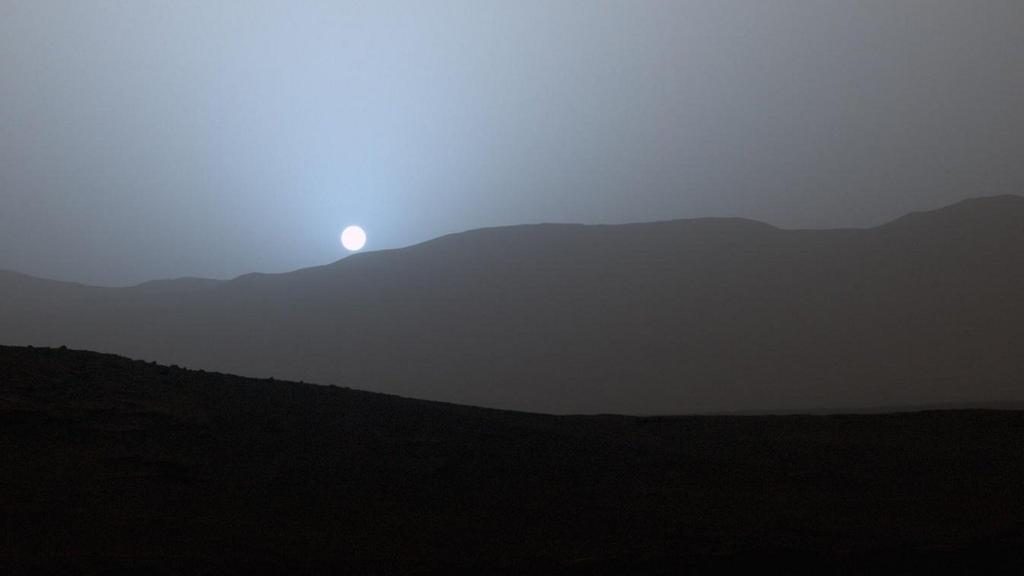
\includegraphics[scale=1.0]{3.jpg}
\label{fig:p0}
\end{figure}





\begin{thebibliography}{99}
\bibitem{2}
Absorption and Scattering of Light by Small Partcicles, Craig F. Bohren, Donald R.Huffman, edit. Wiley-vch, 1998
\end{thebibliography}
\end{document}